\documentclass{article}
\usepackage[letterpaper]{geometry}
\usepackage{graphicx}
\usepackage{xcolor}
\usepackage{amsmath}

% typesetting
% Margins and typesetting
\setlength{\textwidth}{5.00in}
\setlength{\oddsidemargin}{3.25in}
\addtolength{\oddsidemargin}{-0.5\textwidth}
\addtolength{\topmargin}{-0.55in}
\addtolength{\textheight}{2.00in}
\linespread{1.08}
\pagestyle{myheadings}
\markboth{}{\color{gray}\sffamily Hogg \& Villar / \texttt{MNIST-plus-plus}}
\sloppy\sloppypar\raggedbottom\frenchspacing
\renewcommand{\paragraph}[1]{\par\medskip\noindent\textbf{#1} ---}

\title{\bfseries \texttt{MNIST-plus-plus}: Benchmarks for geometric and equivariant learning and reasoning tasks}
\author{David W. Hogg \& Soledad Villar}
\date{}

\begin{document}

\maketitle

\begin{abstract}\noindent
    The objective of this paper is to introduce data, code and benchmarks for simple classification, regression, and reasoning tasks in situations where geometry and geometric symmetries are in play.
    We provide four datasets and seven learning tasks based on simple tranformations of the MNIST and Fashion-MNIST datasets.
    Some of the learning tasks are to recognize objects and handwritten digits in images that have had geometric transformations applied; some are to identify the geometric transformations themselves.
    The images are designed to contain enough context to determine (in most cases) both the image contents and the geometric transformations.
    We train standard-issue CNNs to deliver baseline performances on the learning tasks.
    [SOME SUMMARY OF CNN RESULTS HERE]
    One of the tasks---\texttt{MNIST+4}---involves identifying ordered sets of numbers in a transformed image; it is a true reasoning task and is therefore expected to be challenging for contemporary machine-learning methods.
\end{abstract}

\section{Introduction}

Real-world tasks require us to identify objects in arbitrary orientations and make inferences about their orientations using context. 
See Figure~\ref{fig:example} for example images containing many objects in different orientations.
These images inspire recognition tasks that are interesting from a learning perspective, but also have industrial and commercial uses.
The objective of this contribution is to provide toy datasets that represent baby steps towards general recognition and geometric inference tasks.
These datasets are designed to create benchmarks for learning and reasoning methods.

Individual letters, numbers, and symbols can only be reliably read in certain orientations.
For examples, Ws and Ms, 6s and 9s, ps and ds, 8s and $\infty$s, and so on, cannot be distinguished easily without some understanding of the orientation in which they were written, or intended to be read.
Despite this, when capable human readers pick up pieces of paper with writing or printing on it, they have no trouble orienting them correctly.
How do they orient papers to read them?
They find the orientation that makes the majority of the characters easy to read, in which the writing makes sense or can be used for subsequent tasks.
What would happen if the papers contained only 6s or only Ws?
In this case the papers would not say much of interest!
But they also would be impossible to confidently orient.
So (somehow) it is the diversity of the characters on the page that sets the page orientation.

Individual handwritten digits are the content of what might be the most important benchmark dataset in all of machine learning---the MNIST dataset \cite{mnist}.
As of writing, this dataset has more than XXX citations and many spin-off projects such as spherical-MNIST \cite{spherical}, and Fashion-MNIST \cite{fashion}.
The learning task for MNIST is very simple---identify the handwritten digit from 0 to 9---given oriented, black-and-white thumbnail images.
This task is explicitly \emph{not} an equivariant or geometric task.
All of the digits are given in standard Roman orientations.
Indeed, MNIST recognition projects that enforce invariances or equivariances have the property that they fail to distinguish 6s from 9s, among other pathologies \cite{something}.

In the Real World (tm), printed or captured visual information (letters, digits, images, and symbols) is not always (and maybe not even often) presented to us in an oriented way.
We must orient the print or image before reading it or interpreting it....

BUT: In natural images text can appear with different shears and orientations.
Therefore it is natural to considered a transformed version of MNIST. However, handwritten digits may not be identifiable after rotations or reflections (6s and 9s, 2s and 5s, or even 2s and 6s may look indistinguishable after these transformations).
In natural contexts, however, 6s and 9s are not read in isolation; they are read as part of a document or signage context where orientation can be inferred from surrounding characters and features.
Thus we can make a dataset that is invariant to rotations, but which includes enough contextual information to determine orientations and parities.

We have made four datasets and seven learning tasks, all of which are designed to be swap-in replacements for MNIST and Fashion-MNIST.
RELATIONSHIP to data augmentation?
We have trained some standard CNNs to provide baseline performance on all seven tasks.
These baselines should be easy to crush.

\section{Datasets and learning tasks}

\subsection*{Dataset 1: \texttt{Fashion++}}
The Fashion-MNIST-plus dataset takes the Fashion-MNIST data and subject it to random rotations and reflections. This is a natural classification task since clothing doesn't have a preferred orientation.

\begin{figure}[t!]
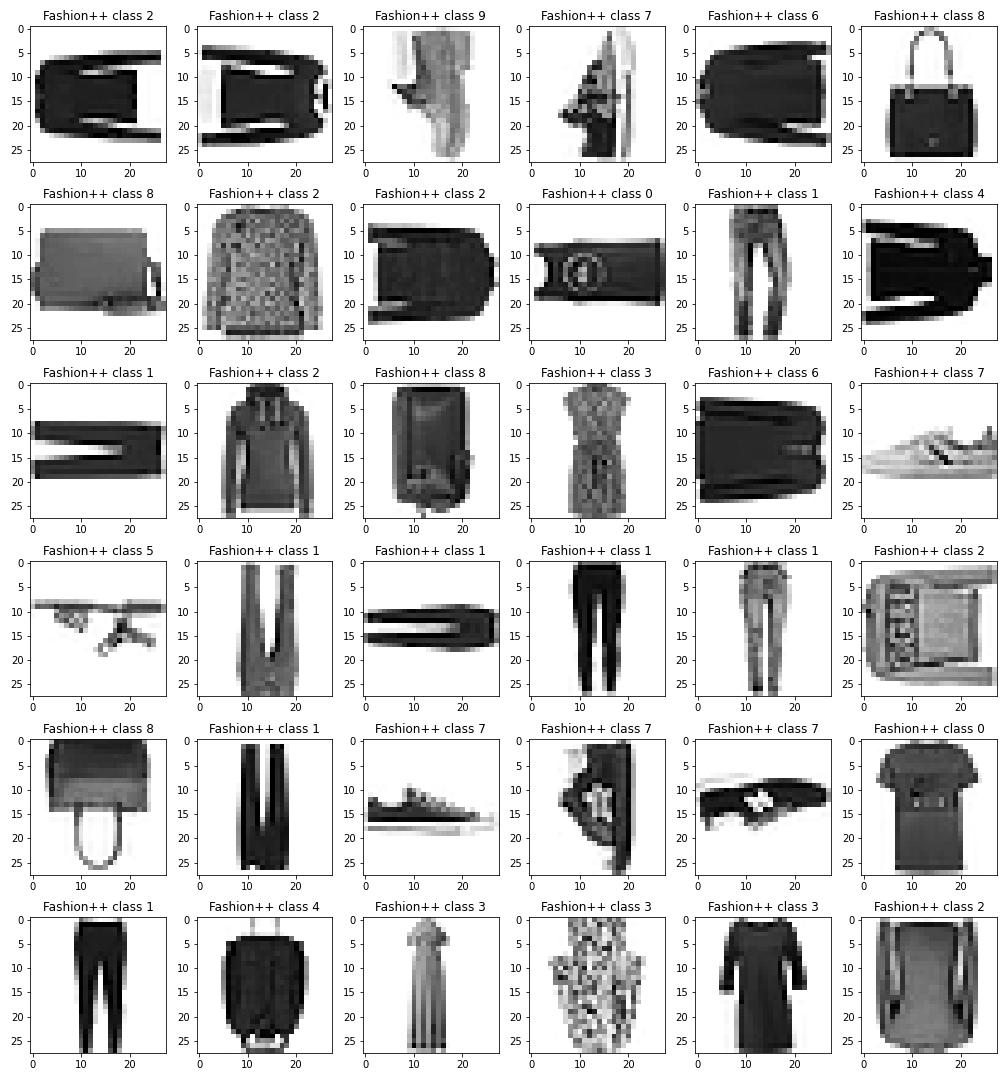
\includegraphics[width=\textwidth]{../notebooks/Fashion++.png}
\caption{The first 36 training-set images from the \texttt{Fashion++} dataset.\label{fig:f}}
\end{figure}

\paragraph{Learning task 1: \texttt{Fashion++} labels}
Identify the labels (classification).

\subsection*{Dataset 2: \texttt{MNIST+4}}

\begin{figure}[t!]
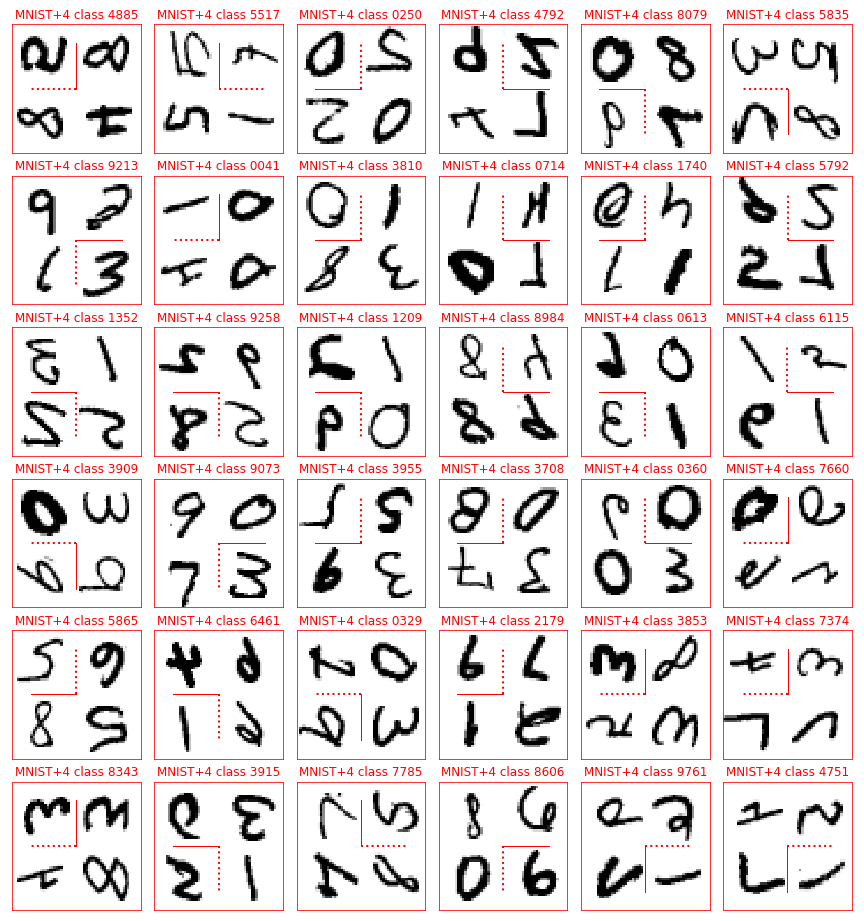
\includegraphics[width=\textwidth]{../notebooks/MNIST+4.png}
\caption{foo and bar.\label{fig:4}}
\end{figure}

\paragraph{Learning task 2: \texttt{MNIST+4} labels}
Identify the labels (classification and reasoning).
This has a reasoning component; note that some labels in the test set don't exist in the training set.
And yet humans can crush this (ish).

\paragraph{Learning task 3: \texttt{MNIST+4} group elements}
Foo and bar.

\subsection*{Dataset 3: \texttt{MNIST+9}}

\begin{figure}[t!]
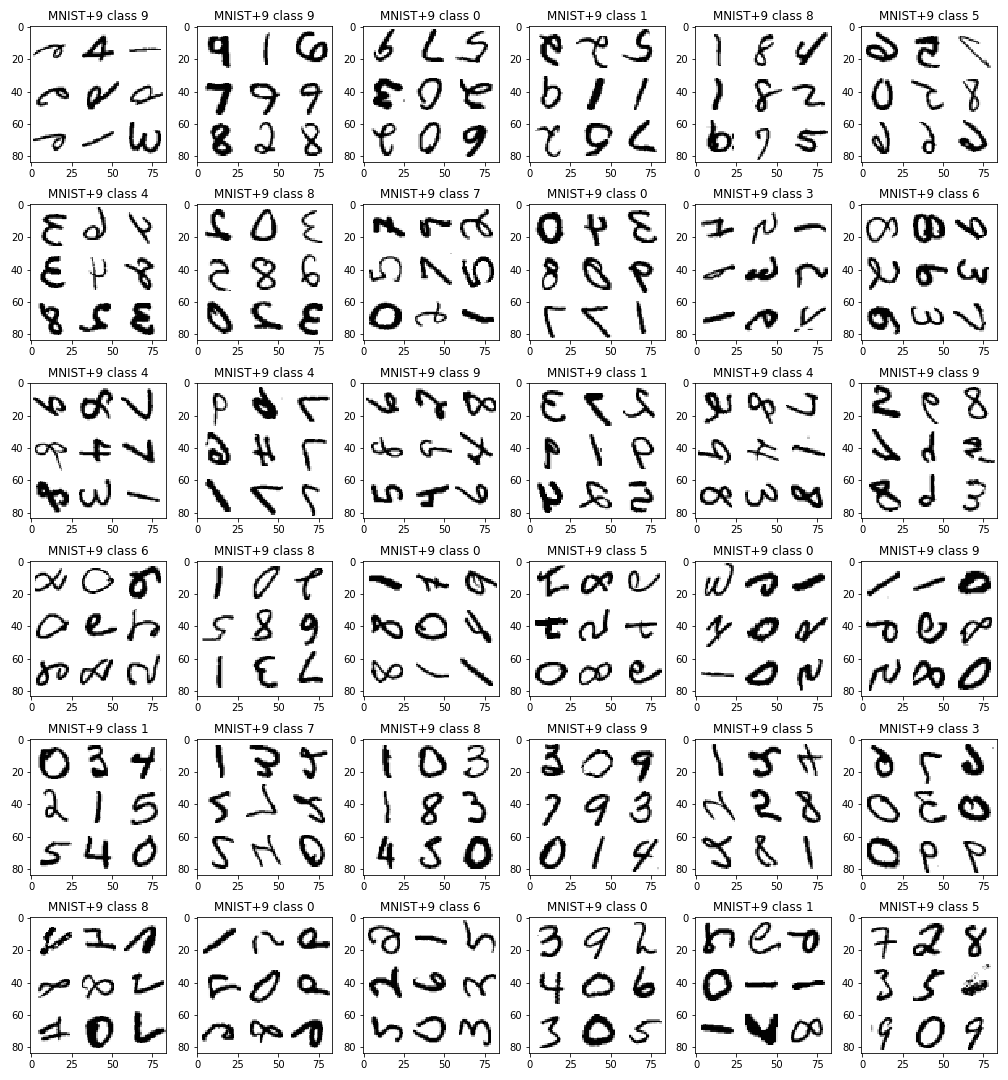
\includegraphics[width=\textwidth]{../notebooks/MNIST+9.png}
\caption{foo and bar.\label{fig:9}}
\end{figure}

\paragraph{Learning task 4: \texttt{MNIST+9} central digit labels}
Identify the labels (classification and reasoning).

\paragraph{Learning task 5: \texttt{MNIST+9} group elements}
Foo and bar.

\subsection*{Dataset 4: \texttt{MNIST+Inf}}

\begin{figure}[t!]
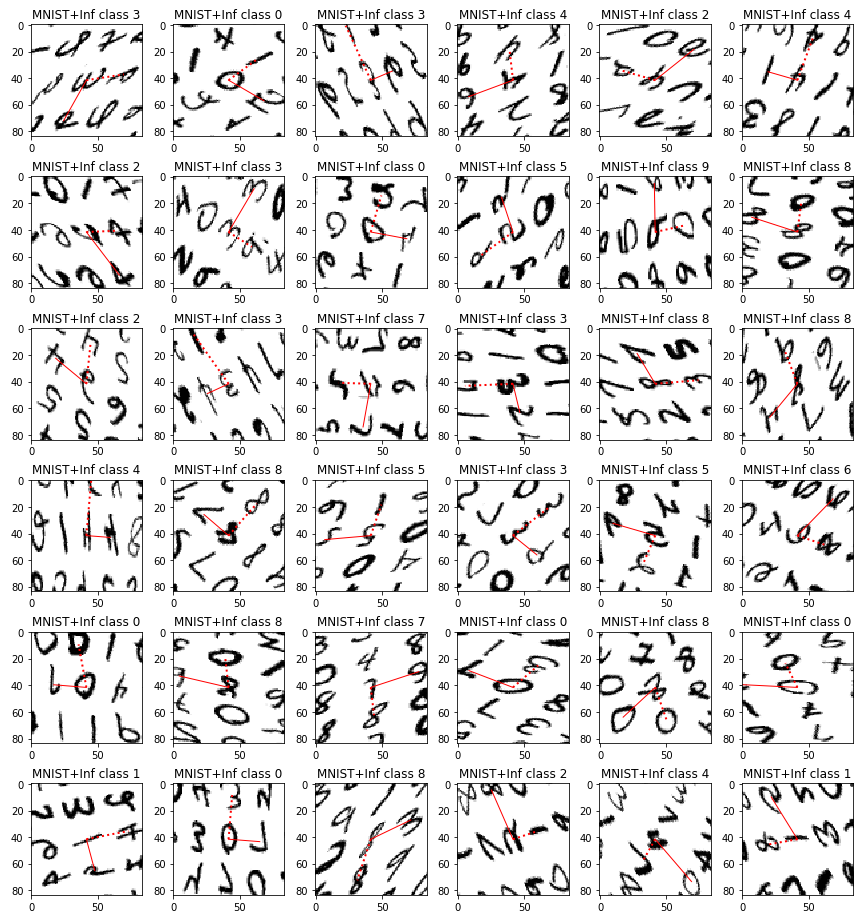
\includegraphics[width=\textwidth]{../notebooks/MNIST+Inf.png}
\caption{foo and bar.\label{fig:Inf}}
\end{figure}

\paragraph{Learning task 4: \texttt{MNIST+Inf} central digit labels}
Identify the labels (classification and reasoning).

\paragraph{Learning task 5: \texttt{MNIST+Inf} linear transformation operators}
Foo and bar. This is a regression!

\section{Baselines}

\section{Data download and discussion}

How do I get the data?

Comments about data augmentation.

Comments about reasoning?

\paragraph{Acknowledgements}
It is a pleasure to thank
  Wilson Gregory (JHU)
for valuable discussions.
SOLE GRANT NUMBERS.

\bibliographystyle{plain}
\raggedright
\bibliography{dipole}

\end{document}
